% !TEX root = ../main.tex
\section{Introduction}
\label{introduction}

An often cited statistic is that data scientists spend at least
$X$\% of their time finding, preparing, integrating and cleaning data sets.
The remaining 100-$X$\% of their time is spent doing the actual desired analysis
tasks.  $X$ is reputed to be 80, 90, 95, or even higher;  in fact,  
a data officer (Mark Schreiber
\eat{\mourad{Maybe, we should add him as a co-author?} }
of Merck) estimates $X$ to 98\%, in which case data
scientists spend less than one hour a week on tasks in their job description.

%----------------------------------
% Positioning Civilzer with respect to other systems early on
% to focus on dcv components more
%----------------------------------------

To address various aspects of this problem, several systems have been developed.  For example, 
  Data Wrangler~\cite{2011-wrangler} and DataXFormer ~\cite{DBLP:conf/icde/AbedjanMIOPS16} automate data preparation by enabled systematic data sources; 
Data Tamer~\cite{DBLP:conf/cidr/StonebrakerBIBCZPX13} attempts to integrate and unify large disparate data sources via schema mappings and record linkage exercises to help scientists work with data sets across silos; 
DeepDive~\cite{DBLP:journals/pvldb/ShinWWSZR15} extract facts and structured information from large corpora of text, images and other unstructured sources.
However, these prior systems all assume that the
data scientist already has a small number of tables he or she wants to clean, integrate, or extract data from, leaving a key challenge unaddressed: finding the data of interest.  Since a typical enterprise data lake contains {\it thousands} of heterogeneous and ill-specified tables, even answering simple questions about where to start looking is hard to do.  

In this paper, we present 
%the architecture of 
\dcv, a system we are building
at MIT, QCRI, Waterloo, and TU Berlin, whose main purpose  is to decrease $X$, by helping data scientists quickly find and query data of interest from large numbers of tables, allowing 
data scientists to spend more of their time on productive data analysis.  We present the main  design requirements of \dcv and the challenges it entails through use cases from the environment at Merck,  a large multi-site drug company with about XXX employees, of which YYY are data scientists.


{\bf[Discovery]} A data scientist at Merck has a hypothesis, for example, {\it the drug Ritalin causes brain cancer in rats weighing more than 1 kg \srm{that's a big rat!}}.  His first job is to identify relevant data sets, both inside and outside of Merck, that might contribute to testing this hypothesis.  Inside the company alone, Merck has approximately  4,000 Oracle databases and countless other repositories.  A {\it Discovery} component in \dcv (cf. Section~\ref{sec:discovery}) has to assist the scientist with finding data sets of interest.

{\bf[Stitching]} The relevant data sets discovered by \dcv  need to be  linked together, often by joining with other intermediary data sets.  Hence, the next step is to construct ``data stitching'' paths among all of the data sets identified during discovery\mourad{Dong, are you getting dataset from outside the discovered set?}\dong{Actually I think discovery the data linkage is also a kind of 'data discovery'. It can be extremely helpful for the users to find the interesting data. Thus I feel we should put data discovery and data stitching side by side in an off-line stage to generate indexes. Then the user can leverage these indexes to find interesting data. Next we can perform fine-grained (but more expensive) stitching and cleaning on the discovered interesting data.}.  We discuss data stitching in detail 
%when we discuss the {\it Data Stitcher} module in \dcv 
in Section~\ref{sec:stitching}. One can think of the output of the data stitcher as views on the underlying data sources. It is now necessary to perform data curation on these views by, for example, extracting data from source data storage systems, performing schema integration on the multiple views, transforming data into a common representation, cleaning erroneous values from the source data sets, and performing entity consolidation on resulting records. Multiple tools, including the tools we mentioned earlier, can be used in tackling these curation and extraction challenges. We have recently evaluated some of the available cleaning tools on multiple data sets~\cite{evaluatioin} to identify the main challenges in this domain.

{\bf[Curation Polystore]} Since Merck has a variety of massive-scale data storage systems, it is  not feasible to move all data to a  central data warehouse. Also, it is not economically, nor technically practical, to perform data curation of all of the thousands of databases up front.
% on the whole available enterprise data. 
 Instead stitching and data curation in \dcv must be done on-demand, as data scientists need to access data to get
their work done.  Therefore, we are building \dcv using a polystore architecture~\cite{DBLP:journals/sigmod/DugganESBHKMMMZ15}, which  can pull data out of multiple underlying storage engines as needed and as dictated by the current analytics task.  Obviously, data cleaning, data transformation and entity consolidation must be integrated with querying the polystore.  In this way, a key technical optimization is to push filters and joins through cleaning operations and into the underlying data storage systems wherever possible.  The
merger of polystores and data curation steps is discussed in Section~\ref{sec:curating}.
%, and we term the resulting system a {\it Curating Polystore}.  

{\bf[Cleanliness Estimation]}  Because of the human effort involved, the expensive processes of creating and curating materialized views  can be very disruptive to the human interaction experience (e.g., validating the view definitions and the stitching results, and validating the automatic cleaning decisions and suggestions).  Therefore, \dcv must estimate the cost of constructing and curating such materialized views  to reason about the feasibility of these operations within the scientists' time budget.  Estimating the cleanliness of a view  entails constructing a model for how dirty the data in the source data sets actually is, which we discuss in Section~\ref{sec:cleanliness}. A related topic is estimating the cleanliness level that can be achieved for a given cleaning budget.  In this way, a scientist can decide
whether or not he wishes to proceed with the project at hand.

{\bf [Optimizing Stitching]} It is highly inefficient and wasteful to  discard expensive-to-construct materialized views after their initial use by a data scientist.  Hence, we assume that they are generally retained for future use.  Moreover, future materialized views  may be based off previously constructed ones or on original data sources.  As a result, there may be several ways to construct a new view, with different  costs and accuracy. Therefore, the data stitching problem must be revisited to deal with this materialization cost/accuracy trade-off.  This is the subject of Sections~\ref{sec:enhancedstitching}.\mourad{Why not merge this section with Data Stitching?}

{\bf [Handling Updates]}  If a source data set is updated, then
updates must be incrementally propagated through the data curation pipeline to
update downstream materialized views.  In some cases, the human effort involved may be
daunting, and the materialized view should be discarded rather than updated.  Lastly, if a
scientist updates a view, we must propagate changes to other derived views, as well as back upstream to data sources, if this is possible. Section~\ref{sec:updates} discusses the update issues and how \dcv handles it.

{\bf [Workflow]} To have end-to-end functionality, \dcv has to offer a workflow engine whereby data scientists can iterate over our components in whatever order they wish; they should also be able to undo previous workflow steps and perform alternate branching from given materialized views. Section~\ref{sec:workflow} discusses the  workflow management in \dcv.

We describe the  current implementation of \dcv  in Section~\ref{sec:wild}, and indicate initial user experience in two use cases: the  MIT data warehouse and Merck. We conclude with final remarks and an  outline of  our future research plans in Section~\ref{sec:conclusion}.


\section{Architecture}
\label{sec:arch}

\dcv adopts the main design principles mentioned in the introduction. %Section~\ref{introduction}. 
It is built as a stack of modules: {\em Discovery}, {\em Stitching}, and finally 
a {\em Query Processing and a Workflow Management} layer. All layers assume a polystore computing environment. Figure~\ref{fig:arch} shows the
general architecture of the \dcv system. 
The discovery layer provides search facilities over the underlying slew of available data sources.
It manages the scale of the underlying data using a high-performance \code{profiler} that
operates on data at different granularities using summarization and statisical profiling techniques.
 Once profiles are build, the discovery engine find related groups of relations using
 measures  such as schema or content similarity;  this is responsibility of the
 \code{graph builder} component. These relationships are
represented in a data fabric similar in spirit to a knowledge graph
\cite{DBLP:conf/semweb/AuerBKLCI07,DBLP:conf/sigmod/BollackerEPST08,DBLP:conf/www/SuchanekKW07}.

The output graph is later used by the stitching layer to find more complex
relationships to stitch these units together and answer a wide range of
analytic queries against ad-hoc schemas. The stitching layer focuses primarily on
exploring the large space of possible ``join relationships'' that connect the
underlying data sets. For example, discovering (often fuzzy) primary key-foreign
key relationships between tables with a \code{cleanliness estimator}. More
generally it extracts inclusion dependencies through the \code{FK-PK refiner},
which allow for joining or stitching these raw data sources together to populate
an analytics schema or a view\mourad{Not sure what an analytics schema/view mean?}. 

The query answering and workflow management layer 
supports the answering of users' queries and composition of user-defined workflows.
%has the goal of answering queries posed by users. 
Queries must be answered despite the heterogeneity and the different levels of
trustworthiness and cleanliness of the underlying sources. This is possible
because the previous layers provide the capability of creating schema views
on-demand for the query to process by using the graph structure populated by
the discovery and stitching layer. To create the right view, a module
called \code{workflow orchestrator} is responsible for coordinating discovery
and stitching. After executing a query (\code{query processor}), the results will
be accompanied of certain quality, which can be improved by, for example,
performing some data cleaning on key tables that contribute to the results. The
module responsible for assessing the result quality and recommending improvement
strategies is called \code{quality controller}.

The  layers in \dcv have different scale and response time constraints,
which greatly affect the design and the choice of algorithms in each layer. 
The discovery layer is ``always on'' working in the background to find, index and
mine connections among large number of data sets, hence, almost-linear
algorithms that work on a Big data scale is a key requirement. 
%On the other hand, 
The stitching layer has to find more complex
relationships, such as inclusion dependencies, which are too expensive to run on
the full scale raw data. Hence, the stitching layer has to judiciously use the
graph output of the discovery layer to scope the search space. While the stitching
layer has an off-line component that focuses on mining these complex join
relationships, efficient use of the query submitted o the query processing layer
can help pruning the large space of possible join graphs. 
Finally, the query processing layer has the tightest response time constraints to respond
within reasonable time to ad-hoc analytics against often continuously changing
analytics schemas (views). Limiting the space of possible data stitching
strategies, while taking into account the polystore execution environment is a
key technical challenge. 

\begin{figure}
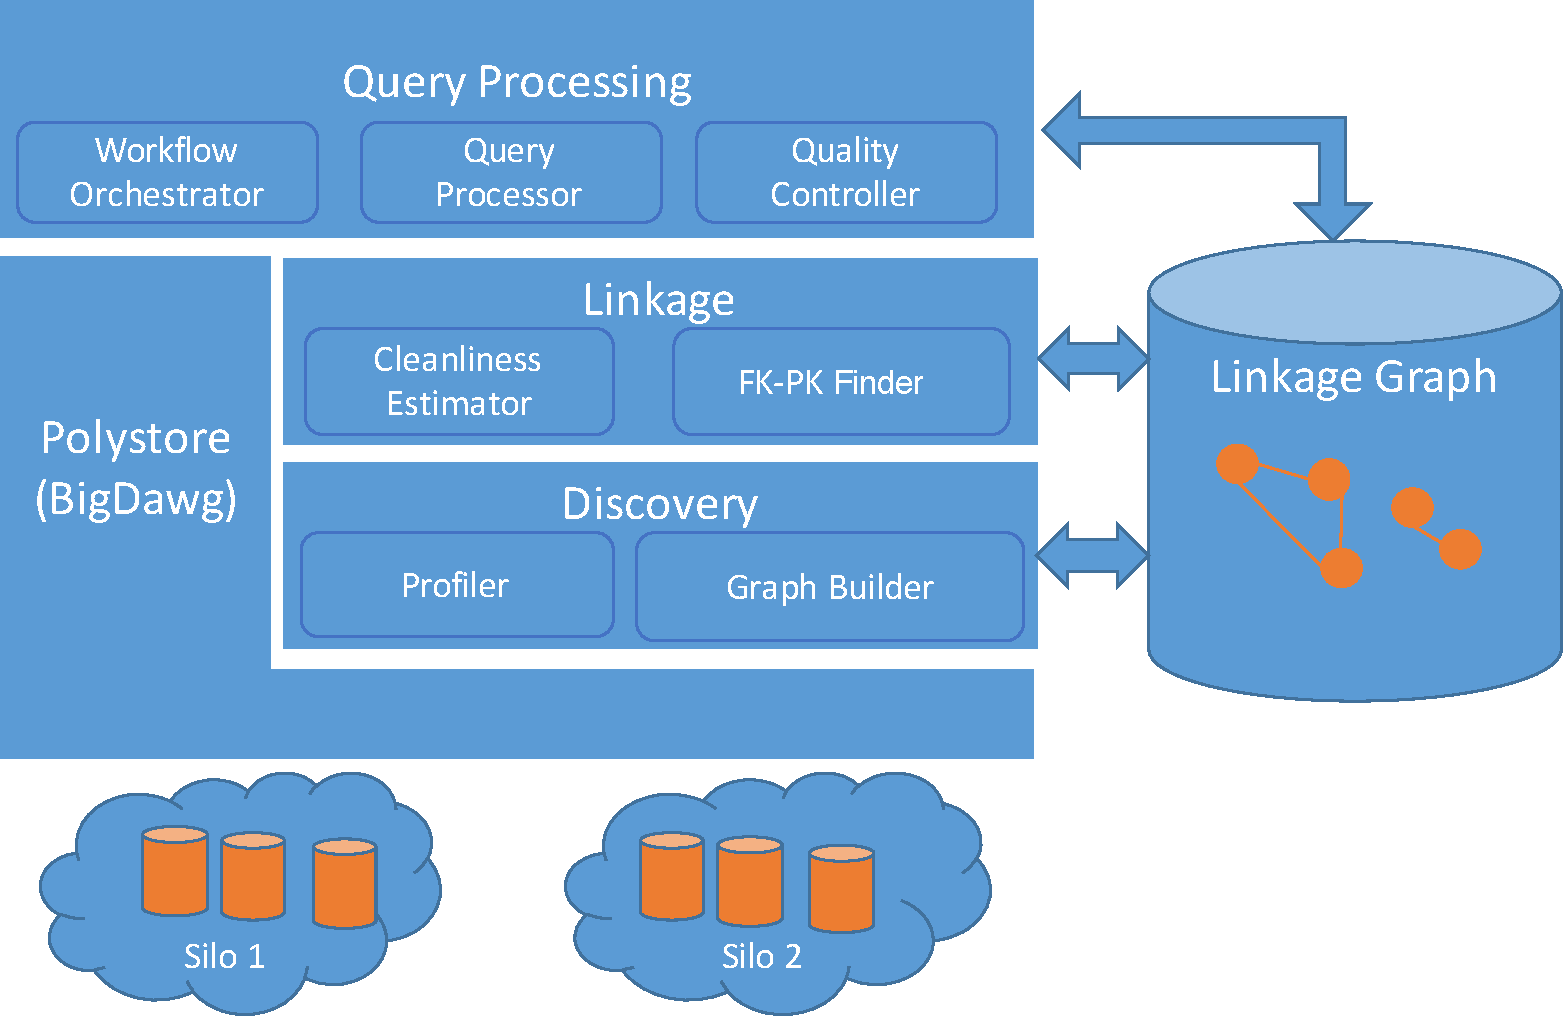
\includegraphics[width=3.5in]{arch3.pdf}
\caption{\dcv Architecture}
\label{fig:arch}
\end{figure}

%\stab \nan{(3): We should merge the concepts of profiles, search path and
%multigraph representation (Section 3), FK-PK (Section 4), and the join graph
%(Section 6) here.}

%\subsection{\nan{\dcv Schema}}
%
%\nan{I would suggest to add here the global schema of \dcv. We need to
%emphasize the followings.}
%
%\stab \nan{(1): \dcv has a schema management module that is different from
%traditional ER-diagram. It has richer semantics. It is highly dynamic.}
%    
%\stab \nan{(2): If the above (1) is agreed, then in Figure 1, the ``Graph
%Builder'' should not be a part of Discovery. Instead, it should be, together
%with stitching Graph, an independent module that supports all the others. I am
%thinking to change this module to be right above the data, but below all the
%other modules.}
%
%\nan{The other Sections can be significantly simplified then.}
